\documentclass[12pt]{article}
\usepackage[a4paper, margin=1in]{geometry}
\usepackage{graphicx}
\usepackage{caption}
\usepackage{parskip}
\usepackage{hyperref}
\usepackage{tikz}
\usepackage{float}

\definecolor{amaranth}{rgb}{0.9, 0.17, 0.31}
%\figureBoxCustom{bottom-left}{top-right}{label}{border-color}
\newcommand*\figureBoxCustom[3]{\draw[#3, ultra thick, rounded corners] (#1) rectangle (#2);}
%\annotatedFigureBoxCustom{bottom-left}{top-right}{label}{label-position}{box-color}{label-color}{border-color}{text-color}
\newcommand*\annotatedFigureBoxCustom[5]{\draw[#5, ultra thick, rounded corners] (#1) rectangle (#2);\node at (#4) [fill=gray,thick,shape=circle,draw=gray,inner sep=2pt,font={\tiny\bfseries\sffamily},text=white] {\textbf{#3}};}

\newenvironment {annotatedFigure}[1]{\centering\begin{tikzpicture}
\node[anchor=south west,inner sep=0] (image) at (0,0) { #1};\begin{scope}[x={(image.south east)},y={(image.north west)}]}{\end{scope}\end{tikzpicture}}

\title{Getting Started with Google Colab}
\date{\vspace{-5ex}}

\begin{document}

\maketitle

\section*{1. What is Google Colab?}

There are many ways to use python, either via a local installation or in the cloud. For the purpose of this course we will be using python via Google Colab (short for "Collaboratory"), which is a free, cloud-based Python editor provided by Google; it allows you to write, run, and save Python notebooks in a web browser, without installing anything on your computer. It's especially useful for beginners and students.

\section*{2. Opening Google Colab and Logging In}

Open your web browser and go to: \url{https://colab.research.google.com}. You'll see a welcome window with a short introduction to Colab.
In order to be able to create new notebboks and save them to Goggle Drive, you will need to sign into your Google account. To do this, you can press the \textbf{“Sign In”} button on the top right. Follow the instructions and fill in your credentials to complete the log in.

\begin{figure}[H]
    \centering
    \begin{annotatedFigure}
        {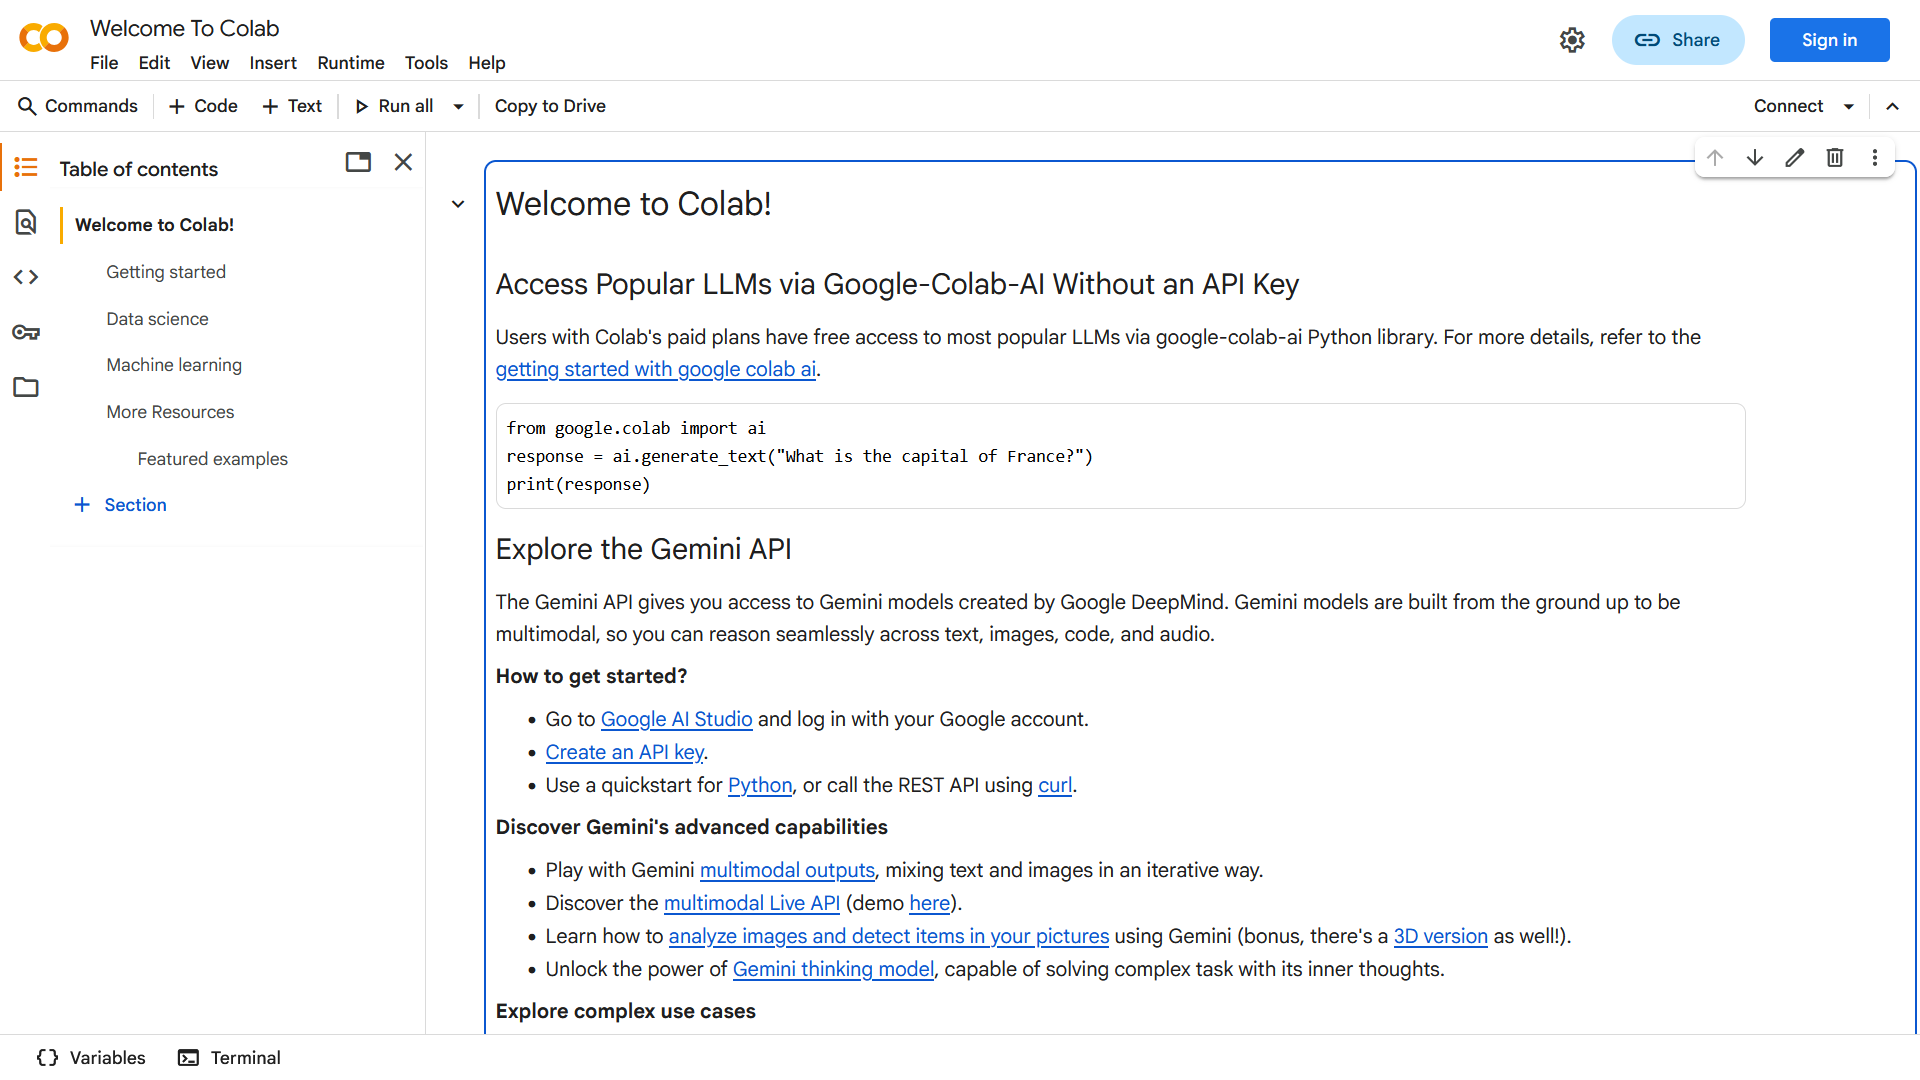
\includegraphics[width=0.85\textwidth]{screenshots/01colab_welcome.png}}
        \figureBoxCustom{0.9157,0.9378}{0.9897,0.9889}{amaranth}
    \end{annotatedFigure}
    \caption{Google Colab welcome page. The Sign In button is on the top right.}
\end{figure}

\begin{figure}[H]
    \centering
	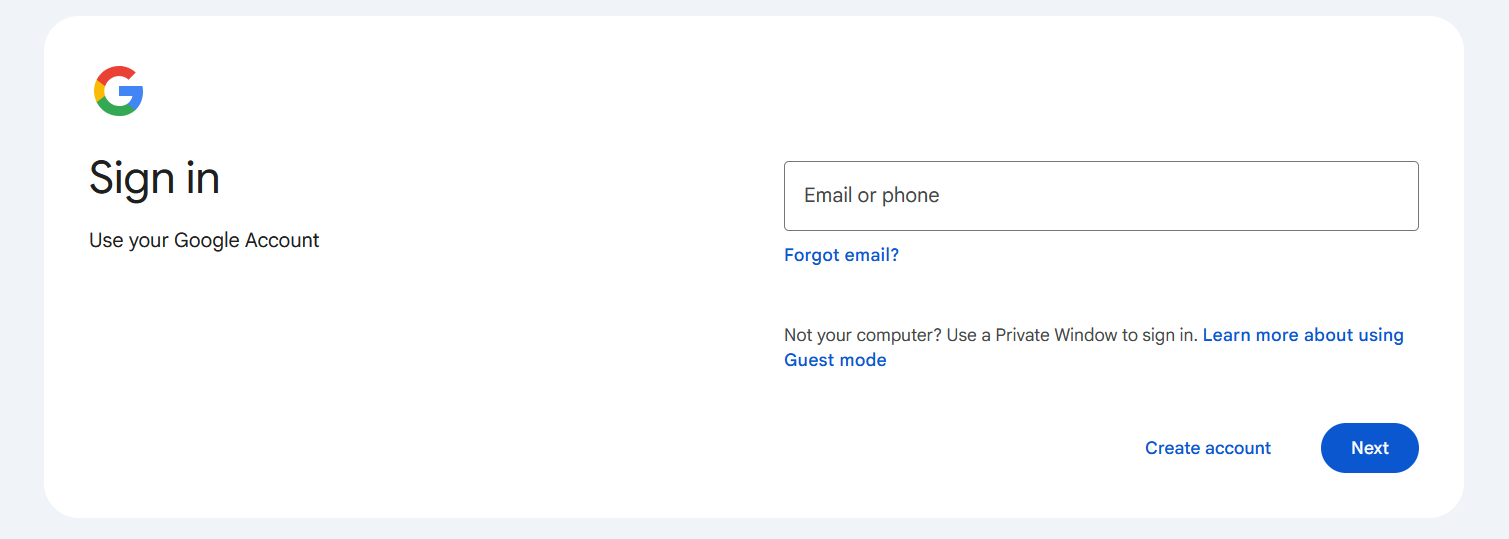
\includegraphics[width=0.85\textwidth]{screenshots/02colab_login.png}
    \caption{Google Log In page.}
\end{figure}

\section*{3. Creating a New Notebook}

Once you're signed in, you can create a new empty notebook by clicking on  \textbf{“File > New Notebook in Drive”} button on the top left; this will save the new notebook in your Google Drive and open it in a new tab at the same time.
\begin{figure}[H]
    \centering
    \begin{annotatedFigure}
        {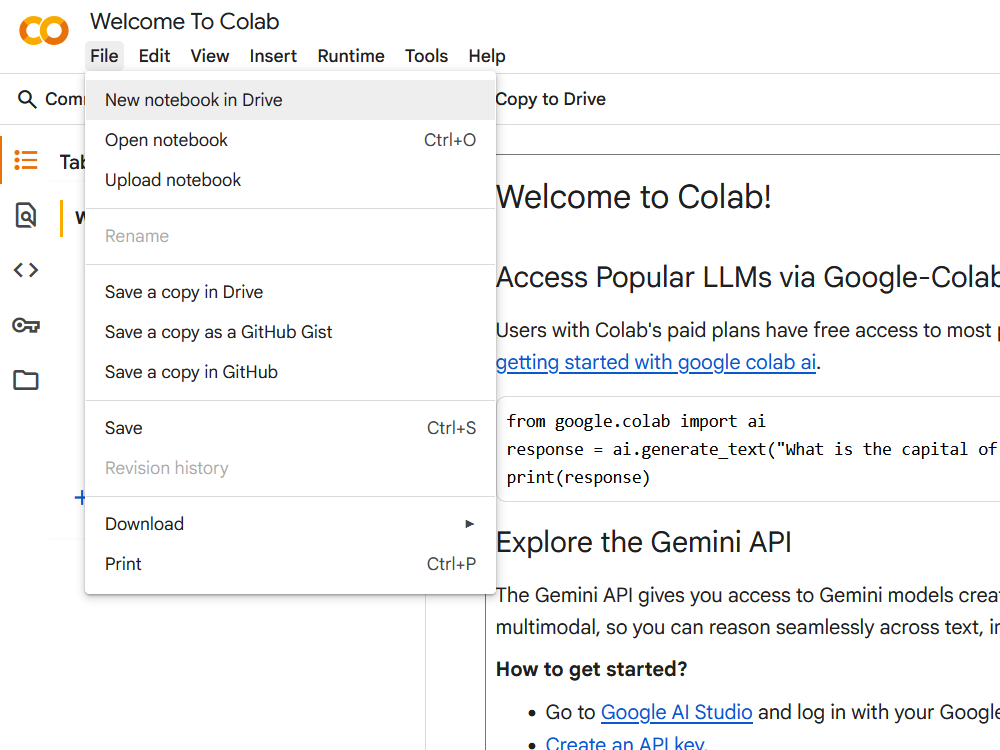
\includegraphics[width=0.85\textwidth]{screenshots/03colab_new_notebook_menu.png}}
        \figureBoxCustom{0.075,0.828}{0.508,0.9053}{amaranth}
    \end{annotatedFigure}
    \caption{New notebook option in \texttt{File} menu.}
\end{figure}

A Notebook is a sequence of cells that contain python statements that can be edited and executed individually.
The result of the evaluation of the statement, be it a string, a number or an image, will be shown below the cell itself.

\section*{4. Understanding the Colab Interface}

Here's a quick overview of the Colab interface:

\begin{enumerate}
    \item \textbf{Toolbar}: at the top — lets you save, run code, add cells, and more.
    \item \textbf{Code Cell}: an area where you can type Python code.
    \item \textbf{Play Button}: to the left of each code cell — click it to run the cell.
    \item \textbf{File Browser}: to the left side menu — allows to load and access additional files.
\end{enumerate}

\begin{figure}[H]
    \begin{annotatedFigure}
        {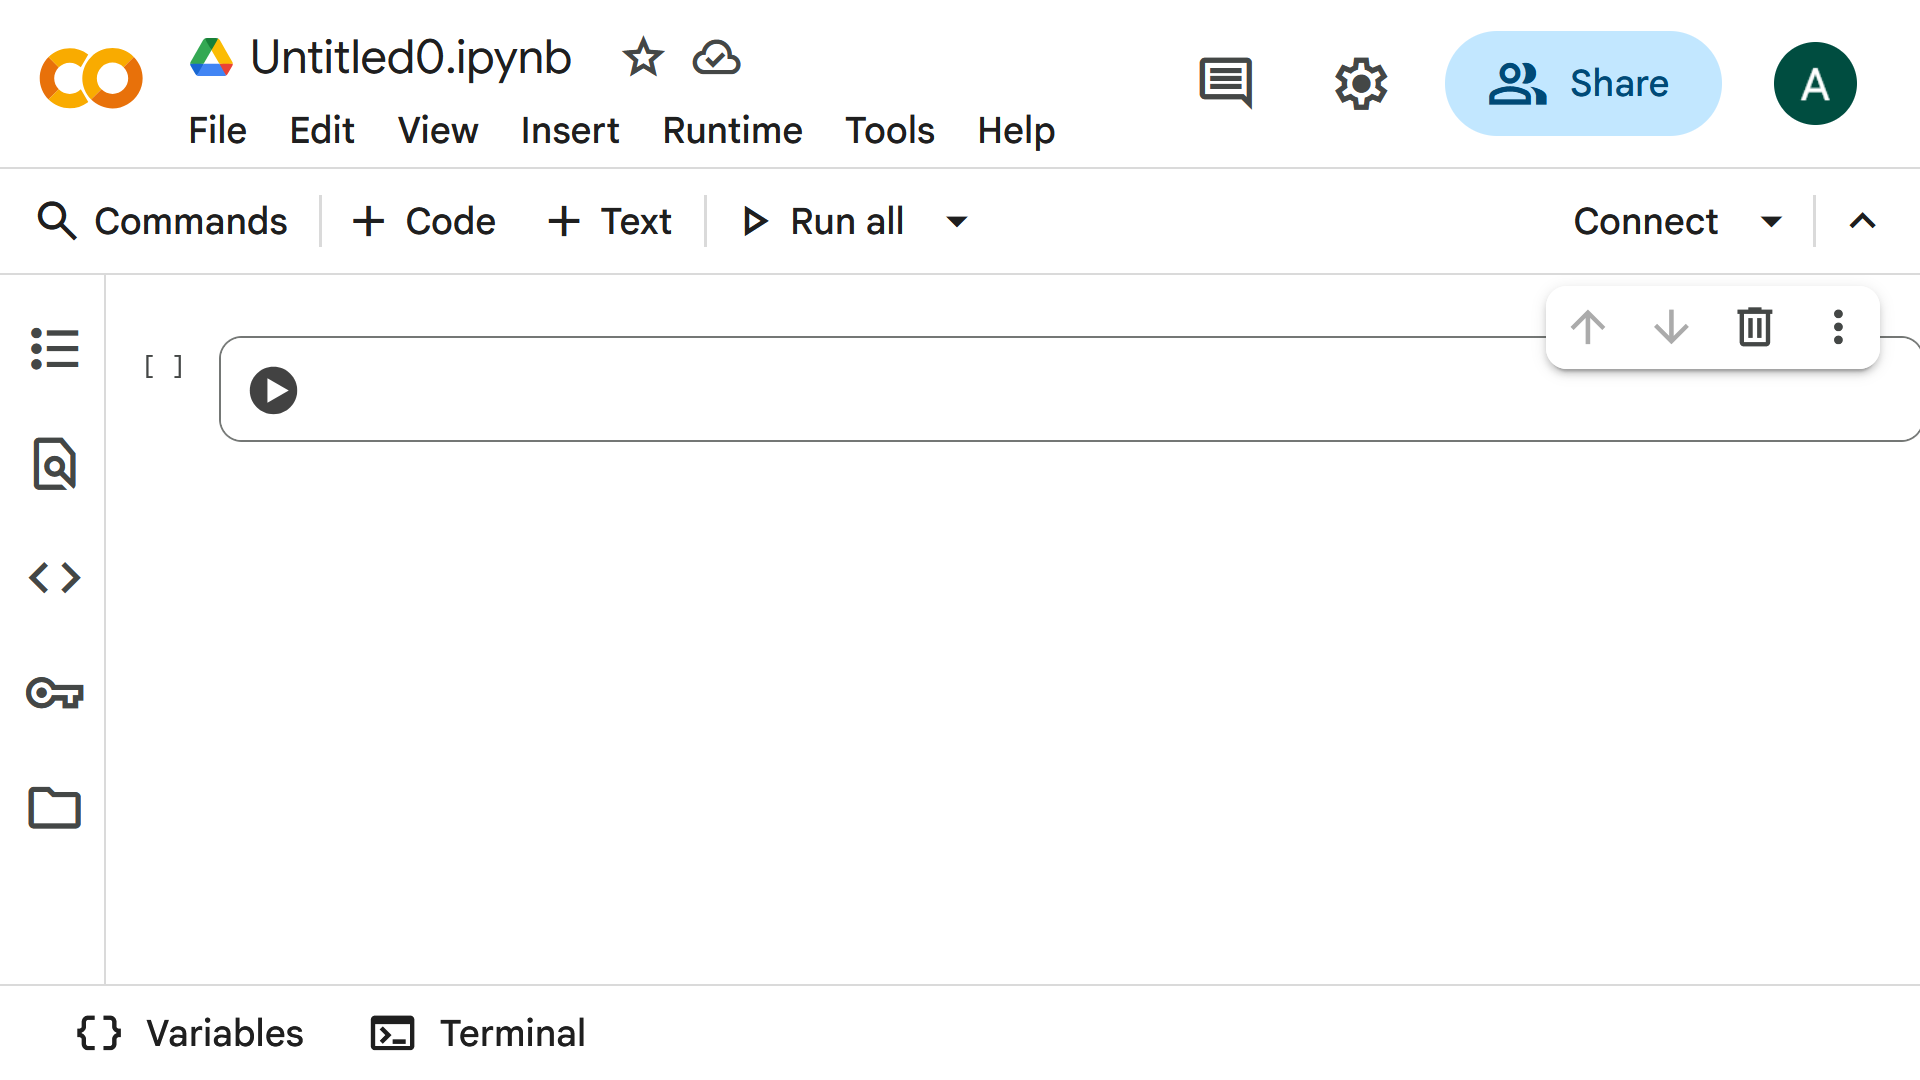
\includegraphics[width=0.85\textwidth]{screenshots/04colab_new_notebook.png}}
        \annotatedFigureBoxCustom{0.038,0.7529}{0.577,0.9147}{1}{0.038,0.7529}{amaranth}
        \annotatedFigureBoxCustom{0.098,0.552}{1.001,0.7191}{2}{0.098,0.552}{amaranth}
        \annotatedFigureBoxCustom{0.122,0.5996}{0.163,0.6782}{3}{0.122,0.5996}{amaranth}
        \annotatedFigureBoxCustom{0.009,0.2138}{0.05,0.2924}{4}{0.009,0.2138}{amaranth}
    \end{annotatedFigure}
    \caption{}
\end{figure}


\section*{5. Writing a Simple Instruction}

Click inside the first cell and type the following Python instruction:

\begin{verbatim}
print("Hello, Colab!")
\end{verbatim}

This line of code will display the text "Hello, Colab!" when run.

\begin{figure}[H]
    \begin{annotatedFigure}
        {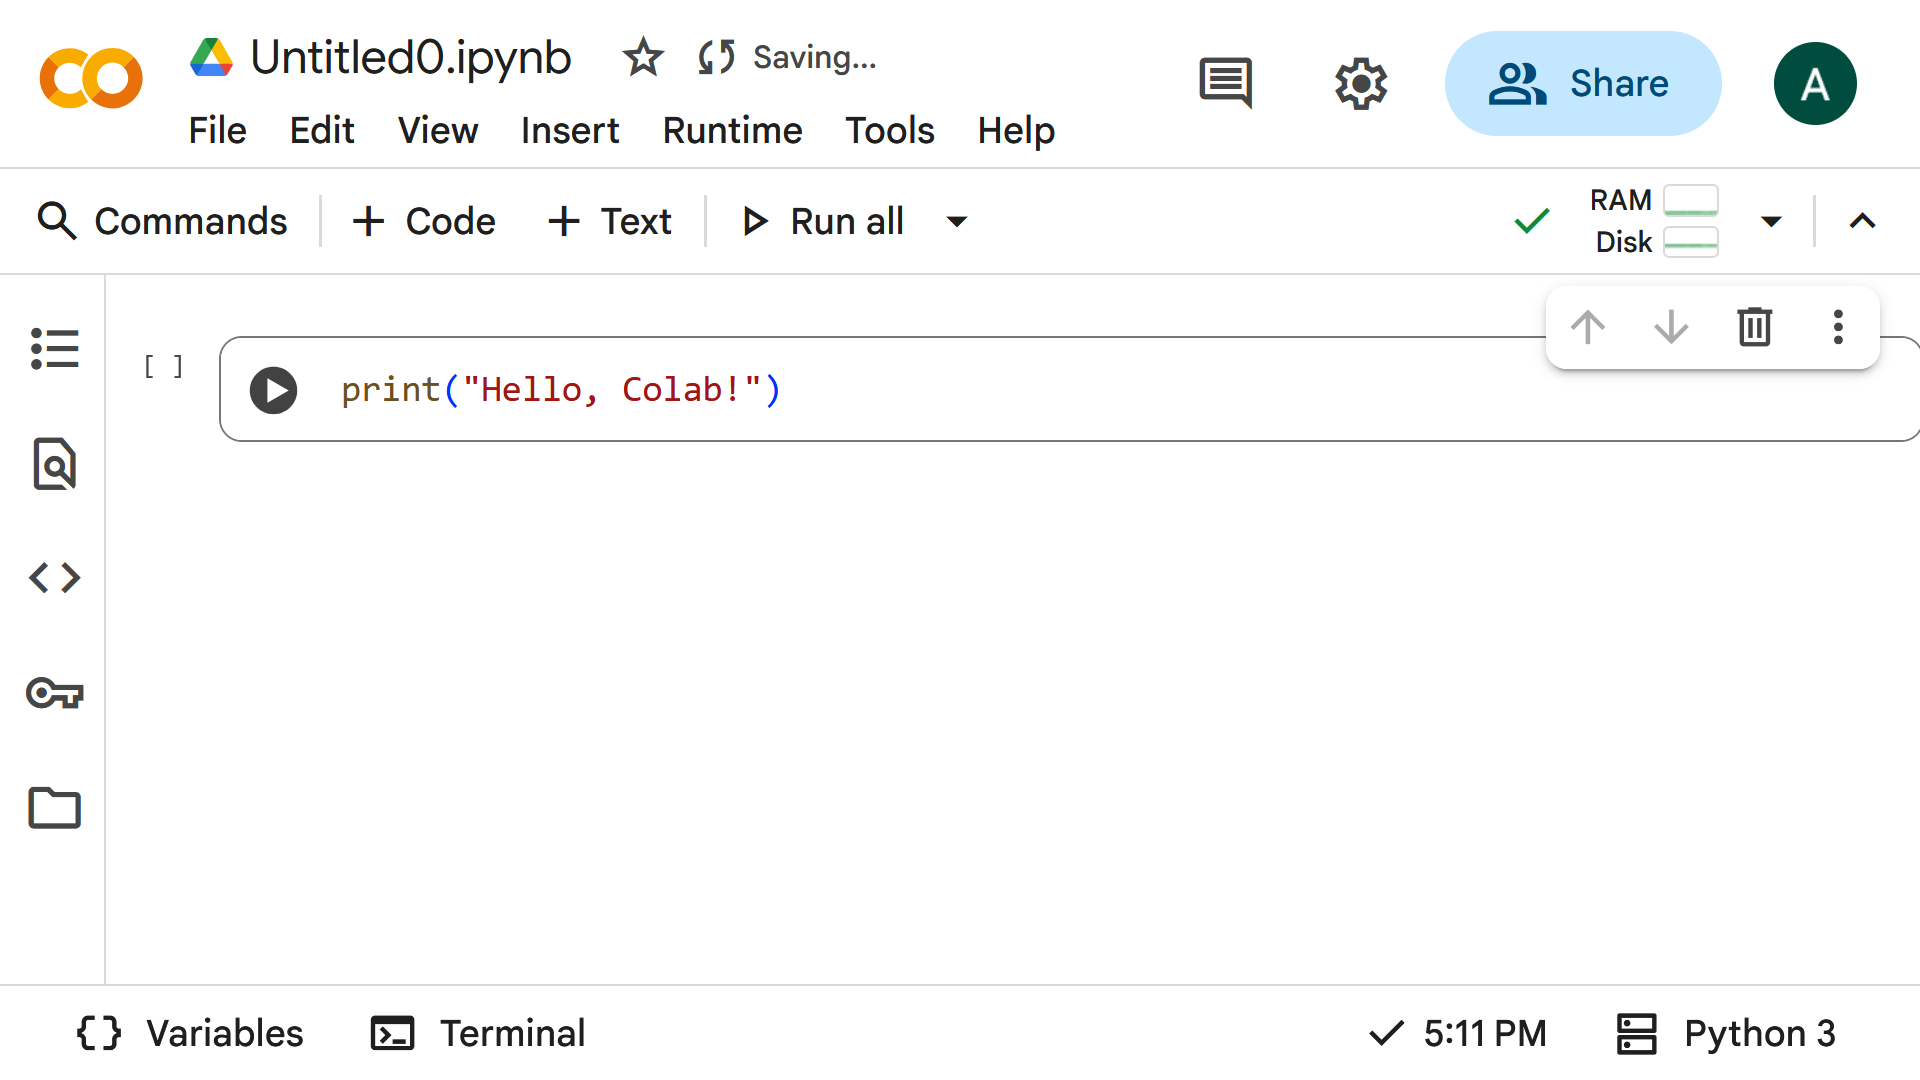
\includegraphics[width=0.85\textwidth]{screenshots/05colab_simple_instruction.png}}
        \figureBoxCustom{0.1621,0.6112}{0.425,0.6702}{amaranth}
    \end{annotatedFigure}
    \caption{Typing a simple print instruction in the first cell of the Notebook.}
\end{figure}

\section*{6. Running a Cell}

To run the cell, you can either:
\begin{itemize}
    \item Click the \textbf{play button} on the left side of the cell, or
    \item Press \texttt{Shift + Enter} on your keyboard.
\end{itemize}
When you run it, Colab connects to a virtual machine in the cloud and executes your code. The output (in this case, the message \texttt{Hello, Colab!}) appears just below the cell.

\begin{figure}[H]
    \centering
    \begin{annotatedFigure}
        {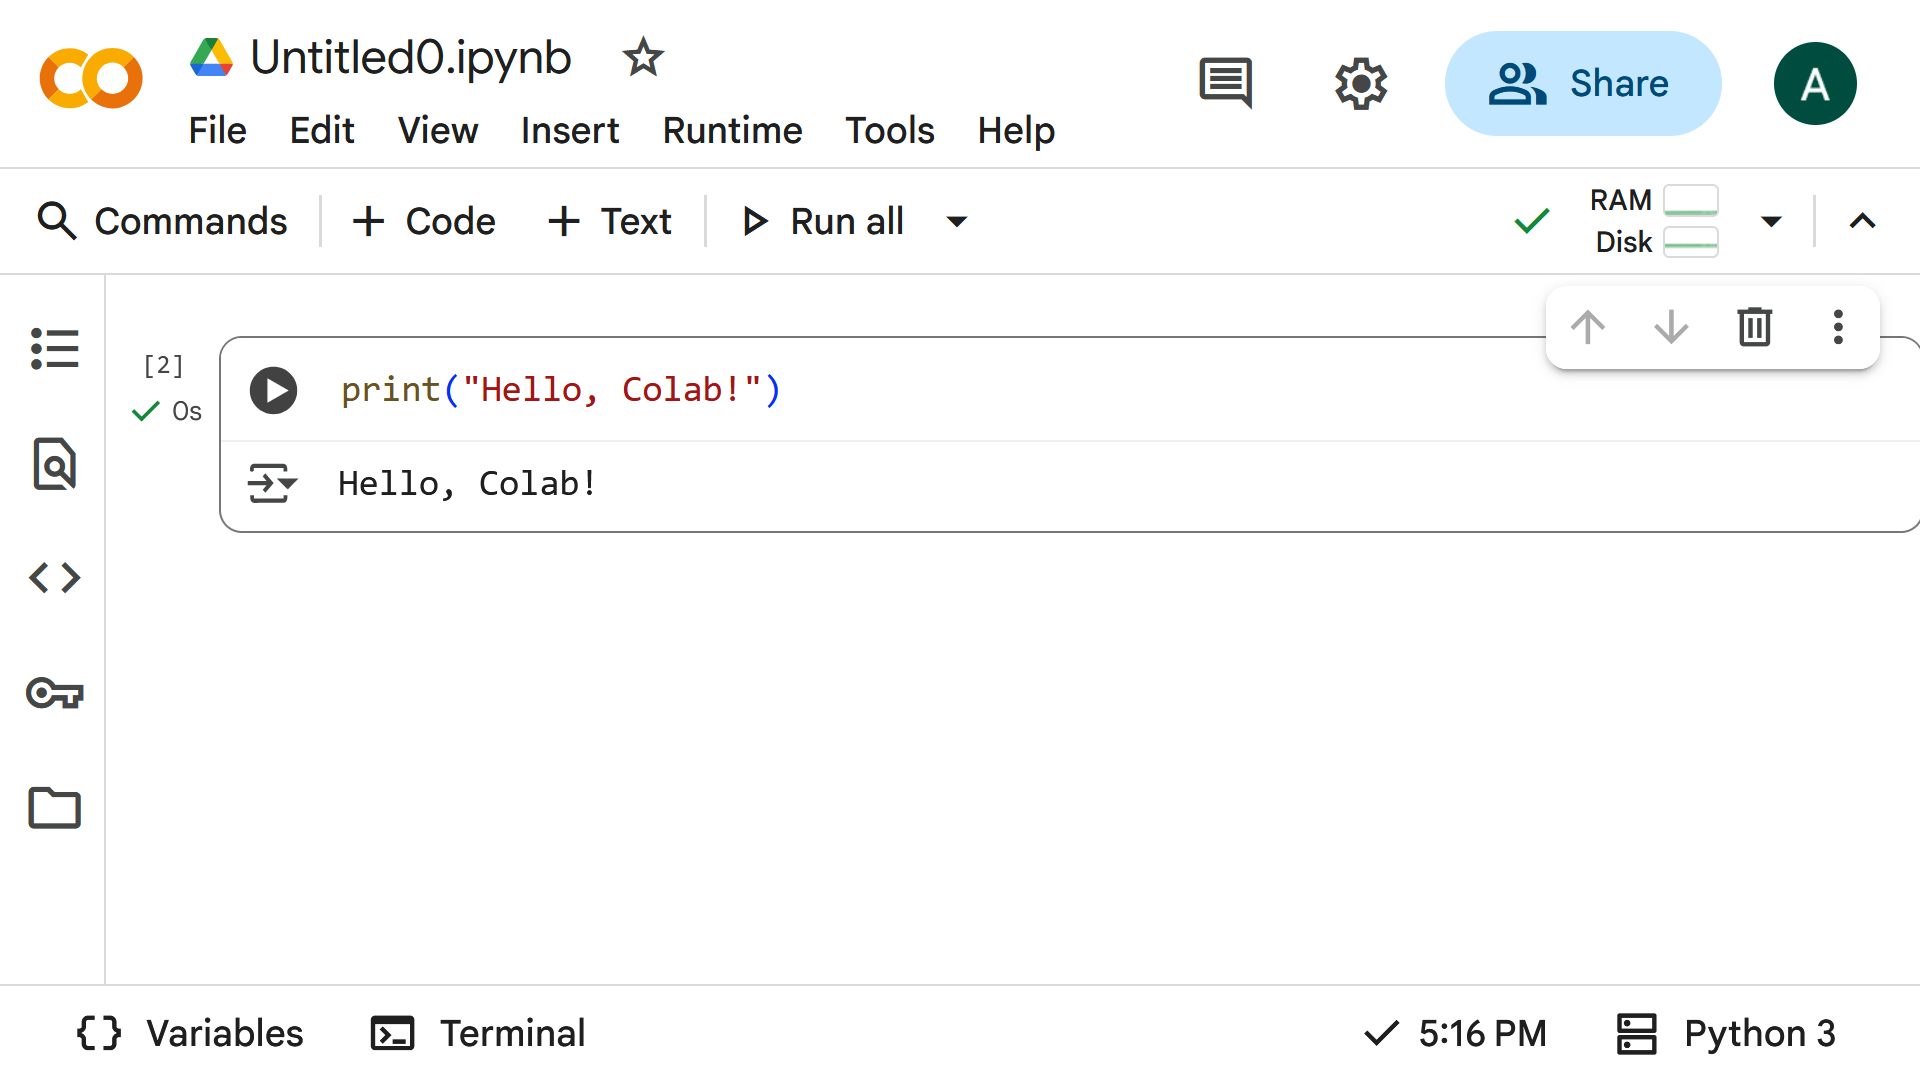
\includegraphics[width=0.85\textwidth]{screenshots/06colab_print_result.png}}
        \figureBoxCustom{0.163,0.5093}{0.322,0.5893}{amaranth}
    \end{annotatedFigure}
    \caption{The result is shown below the cell.}
\end{figure}

\section*{7. Adding New Cells}

To add a new cell to continue writing code, you can:
\begin{itemize}
    \item Click \texttt{+ Code} at the top left or below an existing cell to add a new code cell.
    \item Press \texttt{Shift + M + B} on your keyboard.
\end{itemize}

\begin{figure}[H]
    \begin{annotatedFigure}
        {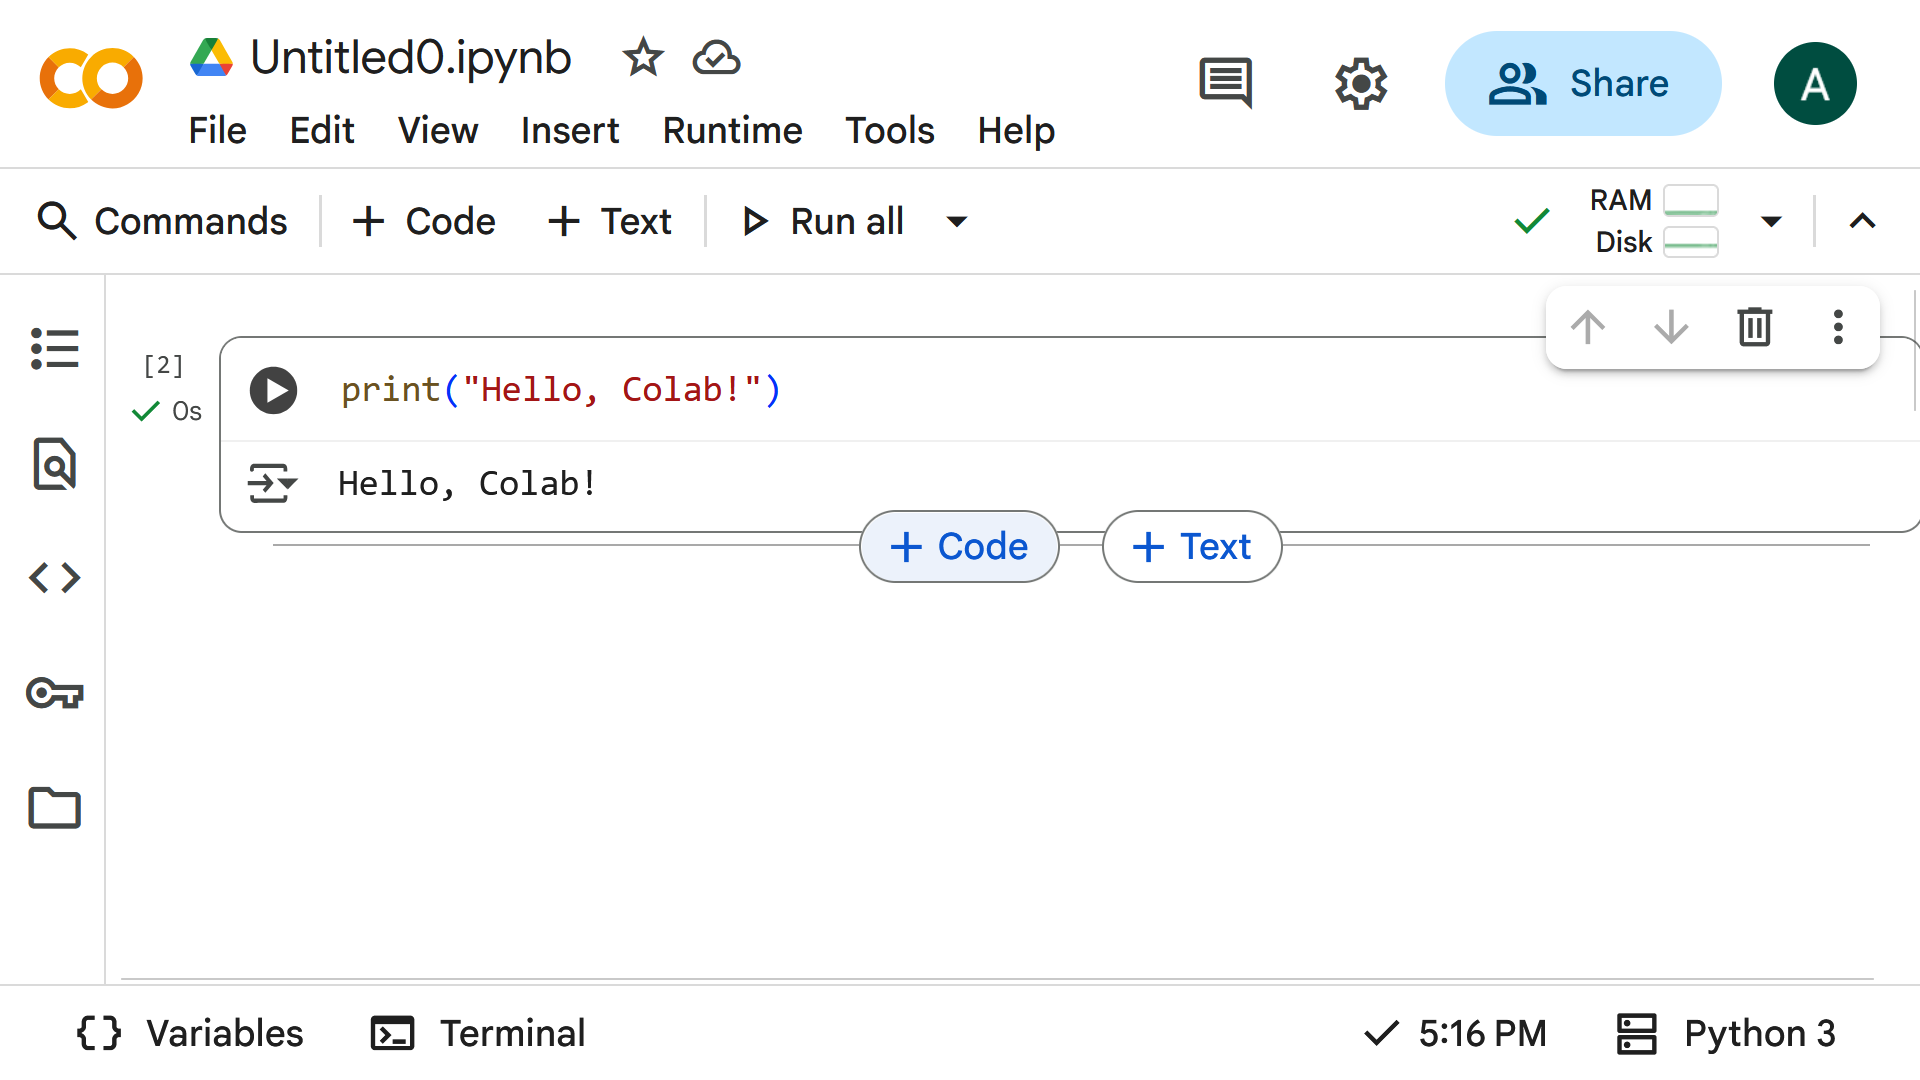
\includegraphics[width=0.85\textwidth]{screenshots/07colab_new_cell.png}}
        \figureBoxCustom{0.175,0.7546}{0.276,0.8346}{amaranth}
        \figureBoxCustom{0.441,0.4489}{0.561,0.536}{amaranth}
    \end{annotatedFigure}
    \caption{Options for creating a new code cell.}
\end{figure}

By clicking \texttt{+ Text} you can instead add a text cell, to add an explanation or comments, uisng plain text or Markdown.

\section*{8. Saving the Notebook}

Colab automatically saves your work in Google Drive whenever you modify it, but you can also manually save by clicking:

\begin{enumerate}
    \item \texttt{File > Save} or press \texttt{Ctrl + S}
    \item Or \texttt{File > Save a copy in Drive} to rename it or save a copy.
\end{enumerate}

The notebook is saved with a \texttt{.ipynb} extension and can be reopened later.

\begin{figure}[H]
    \begin{annotatedFigure}
        {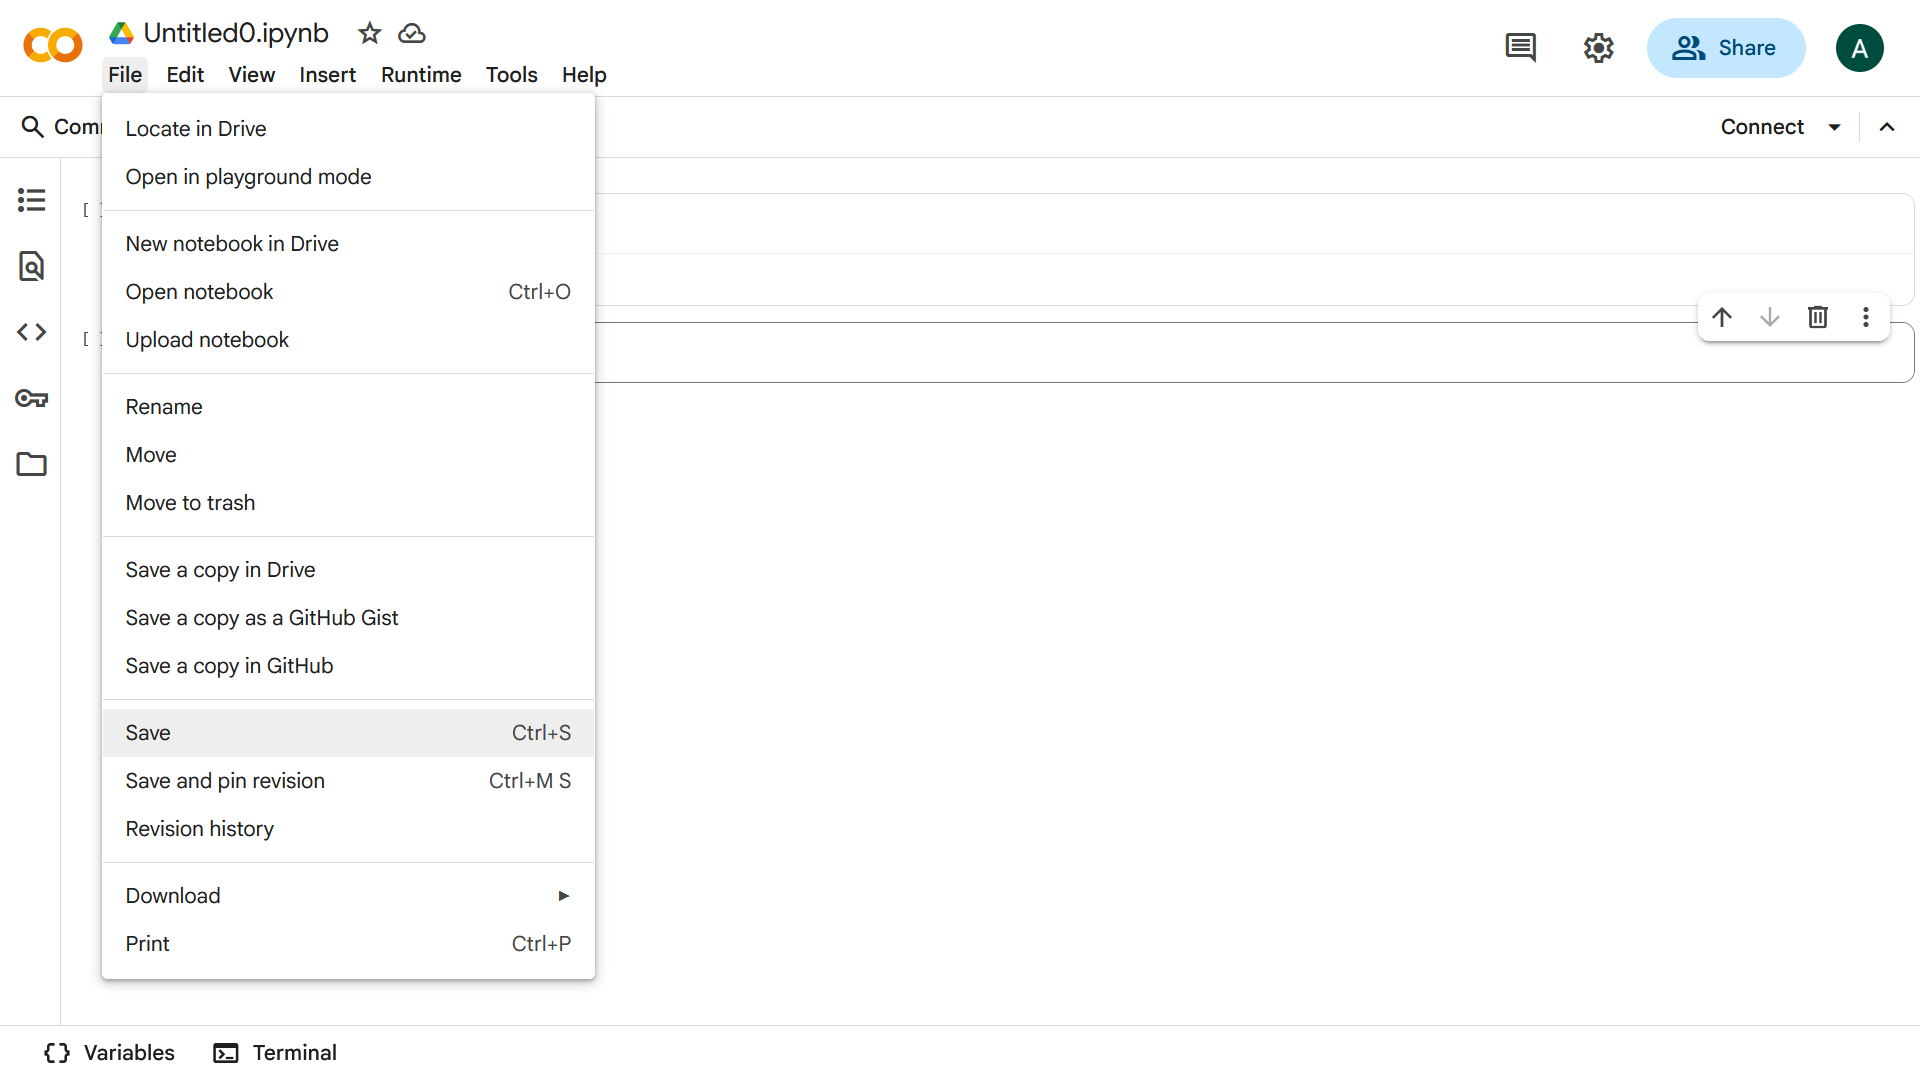
\includegraphics[width=0.85\textwidth]{screenshots/08colab_save.png}}
        \annotatedFigureBoxCustom{0.047,0.2948}{0.315,0.3521}{1}{0.047,0.2948}{amaranth}
	    \annotatedFigureBoxCustom{0.047,0.4424}{0.315,0.4997}{2}{0.047,0.4424}{amaranth}
    \end{annotatedFigure}
    \caption{Save options in \texttt{File} menu.}
\end{figure}

\section*{9. Reopening a Saved Notebook}

To open a saved notebook later, you can either:

\begin{itemize}
    \item Access it directly from your Goggle Drive
    \item Click on \texttt{File > Open notebook} or go back to \url{https://colab.research.google.com} and choose your notebook from the \texttt{"Recent"} or \texttt{"Google Drive"} sections.
\end{itemize}

\begin{figure}[H]
    \begin{annotatedFigure}
        {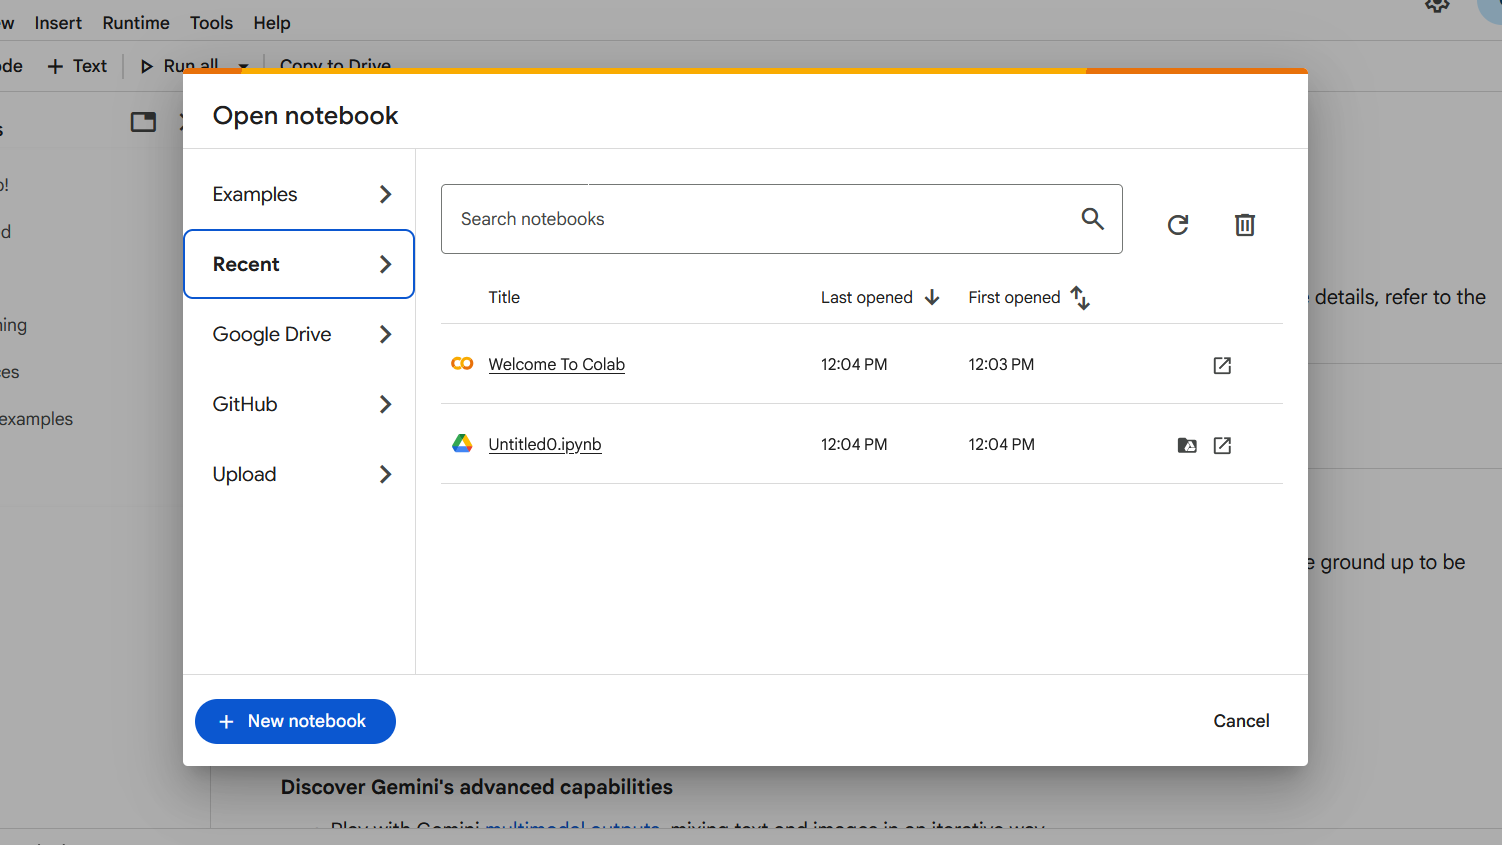
\includegraphics[width=0.85\textwidth]{screenshots/10colab_reopen.png}}
        \figureBoxCustom{0.1301,0.6575}{0.267,0.7165}{amaranth}
	    \figureBoxCustom{0.1301,0.574}{0.267,0.633}{amaranth}
    \end{annotatedFigure}
    \caption{Prompt window that opens when returning to the Colab home page.}
\end{figure}

\end{document}
